% siminos/kittens/cat.tex      pdflatex CL18
% $Author: predrag $ $Date: 2020-09-06 19:08:10 -0500 (Sun, 06 Sep 2020) $

\section{A kicked rotor}
\label{s:kickRot}

The 1-degree of freedom maps that describe kicked rotors
subject to discrete time sequences of angle-dependent impulses
$P(\coord_{\zeit})$, $\zeit\in\integers$,
\bea
\coord_{\zeit+1} &=& \coord_{\zeit}+p_{\zeit+1} \qquad  (\mbox{mod}\;1),
    \label{PerViv2.1b}\\
p_{\zeit+1} &=& p_{\zeit} + P(\coord_{\zeit})
\,,
    \label{PerViv2.1a}
\eea
with $2\pi \coord$ the  angle of the rotor, $p$ the momentum conjugate to
the angular coordinate $\coord$, and the angular pulse
$P(\coord)=P(\coord+1)$ periodic with period $1$, play a key role in the
theory of classical and quantum chaos in  atomic physics, from the
Taylor, Chirikov and Greene  standard map\rf{Lichtenberg92,Chirikov79},
to the cat maps discussed below. The equations are of the canonical
Hamiltonian form: \refeq{PerViv2.1b} is $\dot{\coord}=p/m$ in terms of
discrete time derivative \refeq{lattTimeDer}, \ie, the configuration
trajectory starting at $\coord_{\zeit}$ reaches
$\coord_{\zeit+1}=\coord_{\zeit}+p_{\zeit+1}\Delta{\zeit}/m$ in one time
step $\Delta{\zeit}$, and \refeq{PerViv2.1a} is the time-discretized
$\dot{p}=-\partial V(\coord)/\partial \coord$: at each kick the angular
momentum $p_{\zeit}$ is accelerated to $p_{\zeit+1}$ by the force pulse
$P(\coord_{\zeit})\Delta{\zeit}$, with the time step set to
$\Delta{\zeit}=1$, and the rotor mass $m$ set to 1.

For an atomic physics kicked rotor, the values of the angle $\coord$
differing by integers are identified, but the momentum $p$ is unbounded.
As for the Bernoulli map \refeq{BerStretch}, one compactifies the
momentum by adding $(\mbox{mod}\;1)$ to \refeq{PerViv2.1a}. This reduces
the phase space to a square $[0,1)\times [0,1)$ of unit area, with the
opposite edges identified.

%\section{Life of a single Hamiltonian cat}
\subsection{Cat map}
%    \fi
\label{s:catPV}

The simplest kicked rotor is subject to a force is proportional to
displacement, that is, Hooke's law force $P(\coord)=K\coord$ linear in
the angular displacement $\coord$. The $(\mbox{mod}\;1)$ added to
\refeq{PerViv2.1a} makes the map a discontinuous `sawtooth,' unless $K$
is an integer. In the integer $K$ case, the map
(\ref{PerViv2.1b},\ref{PerViv2.1a}) is of form
 \beq
 \left(\begin{array}{c}
 \coord_{\zeit+1}  \\
   p_{\zeit+1}
  \end{array} \right )=
  \jMps \left(\begin{array}{c}
 \coord_{\zeit}  \\
   p_{\zeit}
  \end{array} \right )\quad (\mbox{mod}\;1)
    \,,  \qquad
 {\jMps} =\left(\begin{array}{cc}
 a & c \\
 d & b
  \end{array} \right)
\,,
\ee{catMap}
where $a,b,c,d$ are integers whose precise values do not matter, as long
as $\det \jMps=1$, \ie, the map is area-preserving. The map is then a
Continuous Automorphism of the Torus, or a {\em `cat map'}, a linear
area-preserving map on the unit 2-torus \statesp, with the field at the
temporal lattice site \zeit,
\(
\ssp_{\zeit} =(\coord_{\zeit},p_{\zeit}) \in  (0,1]\times(0,1]
\)
interpreted as the angular position and its conjugate momentum
at time instant $\zeit$.
    \PC{2020-02-20}{
A matrix $\jMps$  is called hyperbolic when it has no eigenvalue on the unit circle.
    }

We consider the case of stability multipliers
$(\ExpaEig\,,\;\ExpaEig^{-1})$ real, with a positive Lyapunov exponent
$\Lyap >0$,
\beq
\ExpaEig=e^{\Lyap}=(s+\sqrt{(s-2)(s+2)})/2
\,,\qquad
s=\tr{\jMps}=\ExpaEig+\ExpaEig^{-1}
\,.
\ee{StabMtlpr}
The eigenvalues are functions of the single stretching parameter $s$, and
for $|s| > 2$ the cat map \refeq{catMap} is a fully chaotic
Hamiltonian dynamical system. Cat maps with the same $s$ are equivalent
up to a similarity transformation, so it suffices to work out a single
convenient realization, as we shall do here for the \PV\ example
\refeq{eq:StateSpCatMap}.

Cat maps are beloved by ergodicists and statistical mechanicians because,
even though the field $(\coord_{\zeit},p_{\zeit})$ is 2\dmn, for integer
values of the stretching parameter $s$, a cat map has a finite alphabet
linear code, just like the Bernoulli map, and its
unit torus can be tiled by two rectangles (see \reffig{fig:PVAdlerWeiss}\,(a)),
in analogy with the forward-in-time Bernoulli map subinterval
partitioning of \reffig{fig:BernPart}. From this it follows that all
admissible symbol {\brick}s can be generated as shifts of finite
type, and all periodic points determined and counted.

As all that is well known, and a side issue for this paper, we relegate
the details of the Hamiltonian cat map dynamics and \po\ counting to
\refappe{s:catMapHam}. Here we focus on reformulating the cat dynamics as
a temporal lattice (or discrete Lagrangian) problem, as we have done for
the Bernoulli system in \refsect{s:1D1dLatt}.

\subsection{\tempLatt}
\label{s:catLagrange}
    % earlier names:
    % \section{Life of a single Lagrangian cat}
    % \section{Cat map in Lagrangian formulation}
\renewcommand{\period}[1]{{\ensuremath{n_{#1}}}}
    % discrete length of a cycle, Predrag

To motivate our formulation of a \spt\ chaotic field theory to be
developed in \refsect{s:catlatt}, we again recast the local initial
value, time-evolution cat \emph{map} \refeq{catMap} as a global
\emph{temporal lattice} condition that we shall refer to as the
{\em \templatt}.

The discrete time Hamilton's equations
(\ref{PerViv2.1b},\ref{PerViv2.1a}) induce forward-in-time evolution on a
2-torus  $(\coord_{\zeit},p_\zeit)$ {\em phase space}. For the problem at
hand, it pays to go from the Hamiltonian (configuration, momentum) phase
space formulation to the discrete Lagrangian
$(\ssp_{\zeit-1},\ssp_{\zeit})$ formulation. If the momentum is replaced
by the discrete time velocity,
\beq
(\coord_\zeit,p_\zeit) \to
\left(
    \ssp_{\zeit},\frac{\ssp_{\zeit} - \ssp_{\zeit-1}}{\Delta\zeit}
\right)
%\,,\qquad \Delta\zeit= 1
\,,
\ee{Ham2Lagr}
and the time step set to $\Delta\zeit=1$, a cat map can be brought to the
\PV\ `two-configuration representation'\rf{PerViv}
\beq
 \left(\begin{array}{c}
 \ssp_{\zeit}  \\
 \ssp_{\zeit+1}
 \end{array} \right )=
 \jMps_{PV} \left(\begin{array}{c}
 \ssp_{\zeit-1}  \\
 \ssp_{\zeit}
 \end{array} \right ) %\mbox{ mod } 1
 - \left(\begin{array}{c}
 0  \\
 \Ssym{\zeit}
 \end{array} \right )
 \,,  \qquad
 {\jMps_{PV}} =\left(\begin{array}{cc}
 0 & 1 \\
 -1 & s
 \end{array} \right ),
%\,.
\ee{eq:StateSpCatMap}
with matrix $\jMps_{PV}$ acting on the 2\dmn\ space of successive
configuration points $\transp{(\ssp_{\zeit-1},\ssp_{\zeit})}$. As was
case for the Bernoulli map \refeq{1stepDiffEq}, the cat map
$(\mbox{mod}\;1)$ condition \refeq{catMap} is enforced by integers
$\Ssym{\zeit}\in  \A$, where for a given integer stretching parameter $s$
the alphabet \A\ ranges over $|\A|={s}\!+\!1$ possible values for
$\Ssym{\zeit}$,
\beq
\A=\{\underline{1},0,\dots s\!-\!1\}
\,,
\ee{catAlphabet}
necessary  to keep $\ssp_{\zeit}$ for all times $t$ within the unit
interval $[0,1)$. We find it convenient to have symbol
$\underline{\Ssym{}}{}_{\zeit}$ denote $\Ssym{\zeit}$ with the negative
sign, \ie, `$\underline{1}$' stands for symbol `$-1$'. As for the
Bernoulli system, $\Ssym{\zeit}$ can be interpreted as `winding
numbers'\rf{Keating91}, or, as they shepherd stray points back into the
unit torus, as `stabilising impulses'\rf{PerViv}. Here we shall refer to
them as a `code', or, in the field-theoretical parlance, as `sources'.

Written out as a second-order difference equation, the \PV\ map
\refeq{eq:StateSpCatMap} takes a particularly elegant, {\em \templatt}
form
\beq
\ssp_{\zeit+1}  -  s \, \ssp_{\zeit} + \ssp_{\zeit-1}
    =
-\Ssym{\zeit}
\,,
\ee{catMapNewt}
or,
in terms of a {lattice state} $\Xx$, the corresponding {symbol \brick}
$\Mm$ \refeq{pathBern}, and the $[\cl{}\!\times\!\cl{}]$ {\shiftOp}
$\hopMat$ \refeq{hopMatrix},
\beq
(\hopMat - s\unit + \hopMat^{-1})\,\Xx = -\Mm
\,,
\ee{catTempLatt}
very much like the {temporal Bernoulli} condition \refeq{tempBern}.
`Temporal' again refers to the global lattice state (field) $\Xx$, and
the winding numbers (sources) $\Mm$ taking their values on the lattice
sites of a 1\dmn\ \emph{temporal} lattice $\zeit\in\integers$.

For a finite lattice segment $\Xx$, one needs to specify the boundary
conditions ({\bcs}).
%  for the Green's function \refeq{tempCatGreen}.
The companion article \refref{GHJSC16} tackles the Dirichlet {\bcs}, a
difficult, time-translation symmetry breaking, and from the \po\ theory
perspective, a wholly unnecessary, self-inflicted pain. All that one
needs to solve the {\templatt} is the $\period{}$-periodic,
time-translation invariant {\bcs} used here.
    \PC{2020-02-08}{
Complain about that stupidity clearly both in the intro and in conclusions.
    }


\subsection{\JacobianOrb}
\label{s:tempCatJacobianOrb}

Again, the {temporal lattice} reformulation gives us a different perspective
into how to enumerate and determine global solutions of such systems. The
{\templatt} condition \refeq{catTempLatt} can be viewed as a search for
zeros \refeq{tempFixPoint} of the function
\beq
F[\Xx] = \jMorb\Xx+\Mm = 0
\,,
\ee{tempCatFixPoint}
% refer to \ee{tempFixPoint}
with the entire periodic \emph{lattice state} ${\Xx}_{\Mm}$ treated as a
single fixed \emph{point} $(\ssp_1,\ssp_{2},\cdots,\ssp_{\cl{}})$ in the
\cl{}\dmn\ unit hyper-cube $\Xx\in[0,1)^\cl{}$, where
the $[\cl{}\!\times\!\cl{}]$ {\jacobianOrb} $\jMorb$ is now given by
\beq
\jMorb = \hopMat - s\unit + \hopMat^{-1}
% \,.
\ee{tempCatFix}
a tri-diagonal Toeplitz matrix (constant along each diagonal,
$\jMorb_{k\ell} = j_{k-\ell}$) of circulant form,
\beq
\jMorb %  = \hopMat - s\unit + \hopMat^{-1}
  =
\left(\begin{array}{ccccccc}
 -{s}& 1 & 0 & 0 &\dots &0& 1 \\
 1 &  -{s}& 1 & 0 &\dots &0&0 \\
0 & 1 &  -{s}& 1 &\dots &0 & 0 \\
\vdots & \vdots &\vdots & \vdots & \ddots &\vdots &\vdots\\
0 & 0 & \dots &\dots &\dots  & -{s}& 1 \\
 1 & 0 & \dots &  \dots &\dots& 1 &  -{s}
        \end{array} \right)
\,.
\ee{Hessian}

% PC 2020-07-24 turned the former
% \subsection{Hill's formula:
%           stability of an orbit vs. its time-evolution stability}
% \label{s:tempLattHill}
% (that was here) into a separate section Hill.tex

\subsection{Integer lattices}
\label{s:catIntLat}

As in \refsect{s:bernIntLat}, the {\fundPip} given the stretching of the
\cl{}\dmn\ unit hyper-cube $\Xx\in[0,1)^\cl{}$ by the {\jacobianOrb}
counts periodic lattice states, with the {\admissible} lattice states of
period $\period{}$ constrained to field values within
$0\leq\ssp_\zeit<1$. The {\fundPip} contains images of all periodic
lattice states $\Xx_\Mm$, which are then translated by integer winding
numbers $\Mm$ into the origin, in order to satisfy the fixed point
condition \refeq{tempCatFixPoint}. The total number of periodic lattice
states is again, as for the Bernoulli system \refeq{detBern0}, given by
the `fundamental fact'
\beq
N_\cl{} = |\Det\jMorb|
\,.
\ee{detCat0}

Period-1, or fixed point lattice states are easy to count: the
{\jacobianOrb} is a 1\dmn\ matrix, so it follows from
\refeq{catMapNewt} that
\beq
N_1={s}-2
\,,
\ee{catFundPar1}
        \PC{2020-06-10}{to Han:
    If the alphabet \refeq{catAlphabet} is really $|\A|={s}\!+\!1$
    letters, how come there are only ${s}-2$ fixed point lattice states?
    Where did the extra 3 letters go?
        }
        \HL{2020-06-12}{
        The fixed point lattice states with the other 3 letters are not admissible. The fixed point solution satisfies:
        \[
        ({s}-2)\ssp_\zeit = \Ssym{\zeit} \, .
        \]
        Since $\ssp_\zeit \in [0,1)$, the range of \Ssym{\zeit} is $\Ssym{\zeit} \in [0,s-2)$. So the letter $\underline{1}$, $s-2$ and $s-1$ are not in the admissible range, as the corresponding fields of these 3 letters are $-1/(s-2)$, $1$ and $(s-1)/(s-2)$ respectively.
        }

%%%%%%%%%%%%%%%%%%%%%%%%%%%%%%%%%%%%%%%%%%%%%%%%%%%%%%%%%%%%%
% Predrag 2020-02-08 replaced Han's
% {HLLength2Counting}.pdf by hand-drawn catCyc2Jacob.svg
% Han & PC 2020-02-11
% siminos/figSrc/han/Mathematica/CountingFigure/HLLength3Counting.nb
\begin{figure}
  \centering
(a)~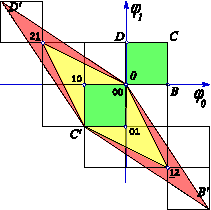
\includegraphics[width=0.38\textwidth]{catCyc2JacobUnit}
~~~
(b)~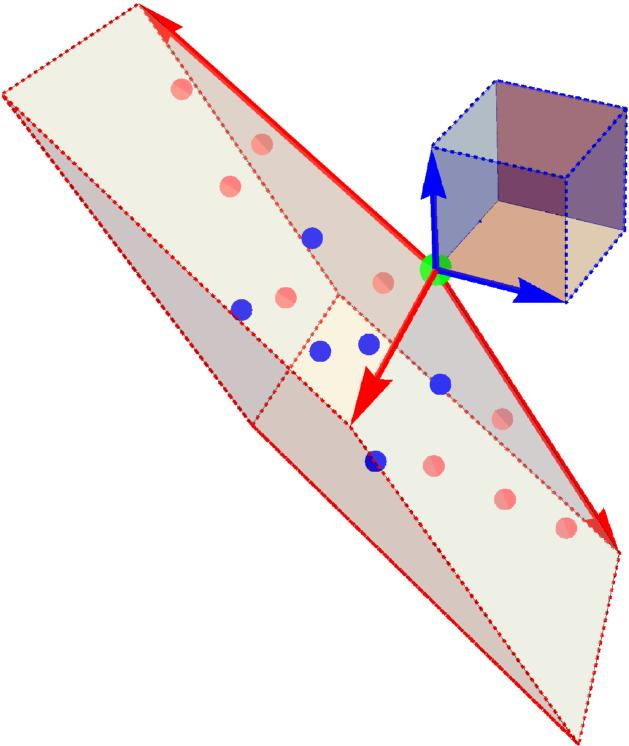
\includegraphics[width=0.34\textwidth]{PCLength3Counting}
  \caption{\label{fig:catCycJacob}
(a)
    For $s=3$, the \templatt\ \refeq{catTempLatt} has 5 period-2 lattice
    states $\Xx_\Mm=(\ssp_0,\ssp_1)$: $\Xx_{00}$ fixed point and
    2-cycles $\{\Xx_{01},\Xx_{10}\}$,
    $\{\Xx_{\underline{1}2},\Xx_{2\underline{1}}\}$. They lie
    within the unit square $[0BCD]$, and are mapped by the
    $[2\!\times\!2]$ {\jacobianOrb} $\jMorb$ \refeq{catFundPar2} into the
    {\fundPip} $[0B'C'D']$, as in, for example, Bernoulli
    \reffig{fig:BernCyc2Jacob}. The images of periodic points $\Xx_\Mm$
    land on the integer lattice, and are sent back into the origin by
    integer translations $\Mm= \Ssym{0}\Ssym{1}$, in order to satisfy the
    fixed point condition
    %\refeq{tempCatFixPoint},
    $\jMorb\Xx_\Mm+\Mm=0$.
(b) A 3-dimensional [{\color{blue} blue} basis vectors] unit-cube stretched by
    $\jMorb$ \refeq{catFundPar3} into the [{\color{red} red} basis vectors]
    {\fundPip}. For $s=3$, the \templatt\
    \refeq{catTempLatt} has 16 period-3 lattice states: a $\Xx_{000}$
    fixed point at the vertex at the origin, [{\color{red} pink dots}] 3
    period-3 orbits on the faces of the {\fundPip}, and
    [{\color{blue} blue dots}] 2 period-3 orbits in its interior.
    An \cl{}\dmn\ unit hyper-cube $\Xx\in[0,1)^\cl{}$ and the
    corresponding {\fundPip} are half-open, as indicated
    by dashed lines, so the integer lattice points on the far corners, edges
    and faces do not belong to it.
}
\end{figure}
%%%%%%%%%%%%%%%%%%%%%%%%%%%%%%%%%%%%%%%%%%%%%%%%%%%%%%%%%%%%%%%

The action of the \templatt\ {\jacobianOrb} is harder to visualize than
the 2\dmn\ {\fundPip} of forward-in-time cat map of
\refappe{s:catHamCount}: a period-2 solution \templatt\ is a 2-torus,
period-3 solution a 3-torus, \etc. Still, the {\fundPip} for the period-2
and period-3 lattice states, \reffig{fig:catCycJacob}, should suffice to
convey the idea. The {\fundPip} basis vectors \refeq{lattJac} are the
columns of $\jMorb$. The $[2\!\times\!2]$ {\jacobianOrb} \refeq{Hessian}
and its {\HillDet} are
\beq
\jMorb =
 \left(\begin{array}{cc}
 -s &  2 \\
  2 & -s
 \end{array} \right)
\,,\qquad
N_2=\Det\jMorb=({s}-2)({s}+2)
\,,
\ee{catFundPar2}
(compare with the lattice states count
\refeq{1stChebGenF}),
with the resulting {\fundPip} shown in \reffig{fig:catCycJacob}\,(a).
The period-3
lattice states for $s=3$ are contained in the half-open {\fundPip} of
\reffig{fig:catCycJacob}\,(b), defined by the columns of $[3\!\times\!3]$
{\jacobianOrb}
\beq
\jMorb =
\left(
\begin{array}{ccc}
-{s}&  1 &  1 \\
  1 &-{s}&  1 \\
  1 &  1 &-{s}
\end{array}
\right)
\,,
\qquad
N_3 = |\Det \jMorb|
%   = {s}^3-3{s}-2
    = ({s}-2)({s}+1)^2
\,,
\label{catFundPar3}
\eeq
again in agreement with the periodic orbit count \refeq{1stChebGenF}.

The 16 period-3 lattice
states $\Xx_\Mm=(\ssp_0,\ssp_1,\ssp_3)$ are the $\Xx_{000}$ fixed point at the
vertex at the origin, 3 period-3 orbits
    $\{
       \Xx_{\Ssym{0}\Ssym{1}\Ssym{2}},
       \Xx_{\Ssym{1}\Ssym{2}\Ssym{0}}
       \Xx_{\Ssym{2}\Ssym{0}\Ssym{1}}
    \}$
on the faces of the {\fundPip}, and 2 period-3 orbits in its
interior.


\subsection{Counting \templatt\ lattice states (unwritten)}
\label{s:tempCatCount}

We now count the number of periodic lattice states \refeq{noPerPts} in
the \templatt\ (or, `discrete Lagrangian') formulation (for counting
using the Hamiltonian formulation, see \refappe{s:catHamCount}).

[...]
one can write
the {\HillDet} compactly as
\beq
N_\period{} = |\det(\jMorb)|
 = 2\,T_{\period{}}(s/2) -2
% = \ExpaEig^{\period{}} + \ExpaEig^{-\period{}} - 2
\,,
\label{POsChebyshev}
\eeq
where $T_{\period{}}(s/2)$ is the Chebyshev polynomial of the first kind.
% end of copied from siminos/spatiotemp/chapter/Green1d.tex

\subsection{Counting \templatt\ lattice states (experimental)}
\label{s:tempCatCountTEMP}
% 2020-06-10 Predrag

The \templatt\ equation \refeq{catMapNewt} is
a linear {$2$nd-order inhomogeneous difference} equation
(a $3$-term recurrence relation) with constant coefficients
%\beq
%\ssp_{\zeit+1}  -  s \, \ssp_{\zeit} + \ssp_{\zeit-1}
%    =
%-\Ssym{\zeit}
%%\,.
%\ee{eq:CatMapNewton2}
that can be solved by standard methods\rf{Elaydi05} that
parallel the theory of linear differential equations.
    \PC{2020-06-10}{
    Comparing with \refeq{genFuncts:CatRec-s} we see that we need to
    solve a second-order inhomogeneous difference equation with a
    constant forcing term $2\,(s-2)$.
    }
Inserting a solution of form $\ssp_{\zeit}=\ExpaEig^\zeit$ into the
associated (\Ssym{\zeit}=0) homogenous {$2$nd-order difference equation}
\beq
\ssp_{\zeit+1} - {s}\,\ssp_{\zeit} + \ssp_{\zeit-1}= 0
\ee{diffEqs:CatCharEq}
yields the {characteristic equation}
\beq
\ExpaEig^{2} - {s}\ExpaEig + 1 = 0
\,,
\ee{diffEqs:StabMtlpr}
which, for $|s|>2$, has two real roots
% stability multipliers
$\{\ExpaEig\,,\;\ExpaEig^{-1}\}$,
\beq
\ExpaEig
% =e^{\Lyap}
=\frac{1}{2}(s+\sqrt{(s-2)(s+2)})
\,,
\ee{PCStabMtlpr}
% fundamental solutions \( \{\ExpaEig^\cl{},\ExpaEig^{-\cl{}}\} \),
and the so-called \emph{complementary} solution of form
\beq
\ssp_{c,\zeit}  = a_1\ExpaEig^\zeit+a_{-1}\ExpaEig^{-\zeit}
\,.
\label{PC(2.3.4)}
\eeq
% where constants $a_i$ can be determined by specifying
% $\{\ssp_{0},\ssp_{1}\}$.

A difference of any pair of solutions to the \templatt\
inhomogenous equation \refeq{catMapNewt}
%\beq
%\ssp_{\zeit+1} - {s}\,\ssp_{\zeit} + \ssp_{\zeit-1}= -\Ssym{\zeit}
%%\,,
%\ee{PC(2.4.4)}
is a solution of the homogenous difference equation
\refeq{diffEqs:CatCharEq}, so the general solution is a sum of the
{complementary} solution \refeq{PC(2.3.4)} and a \emph{particular}
solution $\ssp_{p}$,
\beq
\ssp_{\zeit} = \ssp_{c,\zeit} + \ssp_{p,\zeit}
\,.
\ee{PC(2.4.3)}
Eq.~\refeq{diffEqs:CatCharEq} is time-reversal invariant,
$\ssp_{\zeit} = \ssp_{-\zeit}$, so $a_1=a_{-1}=a$.
To determine the particular solution, assume that both the source
 $\Ssym{\zeit}=\Ssym{}$
and $\ssp_{p,\zeit}=\ssp_{p}$
 in \refeq{catMapNewt} are site-independent,
\beq
\ssp_{p}  -  s \,\ssp_{p} + \ssp_{p}
    = -\Ssym{}
\,,
\ee{eq:CatMapNewton5}
so
\(
%  2\,\ssp_{p}-s\,\ssp_{p}={M}
%  \quad \to \quad
  \ssp_{p} = \Ssym{}/(s-2)
\,.
\)
Hence the solution is
\beq
\ssp_{\zeit} = \ssp_{c,\zeit} + \ssp_{p,\zeit}
= a\left(\ExpaEig^{\zeit} + \ExpaEig^{-\zeit}\right) + {\Ssym{}}/(s-2)
\,,
\ee{Chen11:1stepDiffSolu}
with $a_i$ determined by fields at two lattice sites,
\[
\ssp_{0}= 2a + {\Ssym{}}/(s-2)
\,,\quad
\ssp_{1}= a\left(\ExpaEig + \ExpaEig^{-1}\right) + {\Ssym{}}/(s-2)
\,,\quad
\,.
\]
\tempLatt\ starts with $N_{0}=0$, and according to \refeq{catFundPar1},
$N_{1}=s-2$, so $a=1$, $\Ssym{}=-2(s-2)$, and the number
of temporal lattice states of period $\cl{}$ is
\beq
N_{\cl{}} =
    \ExpaEig^{\cl{}} + \ExpaEig^{-\cl{}} - 2
\,.
\ee{PC:1stepDiffSolu}

\subsection{Shadowing}
\label{s:tempCatShadow}

As the
relation between the symbol {\brick}s $\Mm$  and the corresponding
lattice states $\Xx_\Mm$ is linear, for $\Mm$ an {\admissible} symbol
\brick, the corresponding lattice state $\Xx_\Mm$ is given by
the Green's function
\beq
\Xx_\Mm
= \gd\,\Mm
\,,\qquad
\gd = \frac{1}{-\hopMat + s\unit - \hopMat^{-1}}
\,,
\ee{tempCatGreen}
as in the Bernoulli case \refeq{tempBernGreen}.

As in \refsect{s:bernShadow}, the Green's function \refeq{tempCatGreen}
decays exponentially  with the distance from the origin, a fact that is
essential in establishing the `shadowing' between lattice states sharing
a common sub-\brick\ \Mm. For an infinite temporal lattice
$\zeit\in\integers$, the lattice field at site $\zeit$ is determined by
the sources $\Ssym{\zeit'}$ at all sites ${\zeit'}$, by the  Green's function
$g_{\zeit\zeit'}$ for one\dmn\ discretized heat
equation\rf{PerViv,varcyc},
\beq
  \ssp_{\zeit}=\sum_{\zeit'=-\infty}^\infty g_{\zeit\zeit'} \Ssym{\zeit'}
\,, \qquad
%  g_{\zeit\zeit'} =
%       \left(\frac{1}{-\Box -2 +s}\right)_{\zeit\zeit'}
g_{\zeit\zeit'}=\frac{1}{\ExpaEig-\ExpaEig^{-1}}\,
                \frac{1}{\ExpaEig^{|\zeit-\zeit'|}}
% \,,\qquad
% s=\ExpaEig+\ExpaEig^{-1}
\,,
\ee{1dLatGreenFct}  %{Coord}
with $\ExpaEig$ is the expanding stability
multiplier defined in \refeq{StabMtlpr}.

Suppose there is a non-vanishing point source $\Ssym{0}\neq0$ only at the
present, $\zeit'=0$ temporal lattice site. Its contribution to
$\ssp_{\zeit}$ $\sim \ExpaEig^{-|\zeit|}$ decays exponentially  with the
distance from the origin. More generally, as in the Bernoulli case
\refeq{Bern_cyc}, if two lattice states $\Xx$, $\Xx'$ share a common
sub-\brick\ \Mm\ of length \cl{}, they shadow each other with accuracy of
order of $O(1/\ExpaEig^{\cl{}})$.

\subsection{\Tzeta}
\label{s:tempCatZeta}

The number of lattice states of period $\cl{}$ is
given by the area of the {\fundPip} \refeq{detCat0}
%\rf{Isola90,Keating91}
\beq
N_{\cl{}} = |\Det\jMorb|
          = |\det(\jMps^{\cl{}} - \matId)|
          = \ExpaEig^{\cl{}} + \ExpaEig^{-\cl{}} - 2
\,,
\ee{noPerPts}
where the $\ExpaEig$ is the stability multiplier \refeq{StabMtlpr} of the
one-time-step evolution matrix $\jMps$ \refeq{catMap}.

Substituting the numbers of lattice states $N_{\cl{}}$ into the {\em
{\tzeta}} \refeq{topoZeta} we obtain
\index{topological!zeta function}
\index{zeta function!topological}
\index{Artin-Mazur zeta function}
\index{zeta function!Artin-Mazur}
\bea
\zetatop(z)
 &=& \exp \left(-\sum_{\cl{}=1}^\infty
\frac{z^\cl{}}{\cl{}} N_\cl{}
         \right)
 =  \exp \left(-\sum_{\cl{}=1}^\infty
\frac{z^\cl{}}{\cl{}} (\ExpaEig^\cl{} + \ExpaEig^{-\cl{}} - 2)
         \right)
\continue
 &=&
\exp \left[\ln(1 - z \ExpaEig) + \ln(1 - z \ExpaEig^{-1}) - 2 \ln(1 - z) \right]
\continue
 &=&
\frac{(1 - z \ExpaEig)(1 - z \ExpaEig^{-1})}{(1 - z)^2}
 =
\frac{1 - s z + z^2}
     {(1 - z)^2}
\,,
\label{Isola90-13}
\eea
in agreement with Isola\rf{Isola90}, as well as the \AW\ generating
partition \tzeta\ \refeq{Isola90-13a}. \Tzeta s count {\em prime
orbits}, \ie, time invariant \emph{sets} of equivalent lattice states
related by translations (cyclic permutations), and other
symmetries\rf{CBcount}.

Conversely, given the \tzeta, the generating
function for the number of temporal lattice states of period $\cl{}$ is
given by the logarithmic derivative of the {\tzeta} \refeq{zetatop-N},
\bea
\sum_{{n}=0}^\infty N_{n} z^{n}
    & = & \frac{2-{s}z}{1 - s z + z^2}-\frac{2}{1 - z}
    \continue
& = & (s-2)\left[z + ({s}+2) z^2 + ({s}+1)^2 z^3 \right.
    \ceq
      \left.\qquad\quad
      +\,({s}+2)\,{s}^2 z^4 + (s^2+ s-1)^2 z^5  +  \cdots\right]
\,,
\label{1stChebGenF}
\eea
which is indeed the generating function for $T_{\period{}}(s/2)$, the
Chebyshev polynomial of the first kind of \refeq{POsChebyshev}.

\subsection{\tempLatt\ as a continuous time dynamical system}
\label{s:tempCatODE}

Recall how the Bernoulli first-order difference equation could be viewed as
a time-discretization of the first-order linear ODE \refeq{1stepVecEq}. The
second-order difference equation \refeq{catMapNewt} can be interpreted as the
second order discrete time derivative ${d^2}/{dt^2}$, or the temporal
lattice Laplacian,
\beq
\Box \, \ssp_\zeit \equiv
\ssp_{\zeit+1} - 2\ssp_{\zeit} + \ssp_{\zeit-1}
= (s-2)\ssp_{\zeit} -\Ssym{\zeit}
\,,
\ee{PerViv2.2}
 with the time step set to $\Delta\zeit=1$.
But that is nothing but Newton's Second Law: ``acceleration equals
force,'' so Percival and Vivaldi\rf{PerViv} refer to this formulation as
`Newtonian', while Allroth\rf{Allroth83}, Mackay, Meiss, Percival, Kook
\& Dullin\rf{meiss92,MacMei83,MKMP84,DulMei98,kooknewt}, and Li and
Tomsovic\rf{LiTom17b} refer  to it as the `Lagrangian' formulation.
%, \refsect{s:catLagrForm}.

In other words, for a cat map the force pulse $P(\coord)=(s-2)\,\coord$
in \refeq{PerViv2.1a} is linear in the angular displacement $\coord$, so
the temporal lattice equation takes form
\beq
(\Box -(s-2)\unit)\,\Xx =-\Mm
%    \,,  \qquad
% \Box\,\ssp_{\zeit}:= \ssp_{\zeit-1}-2\ssp_{\zeit} +\ssp_{\zeit+1}
\,.
\ee{OneCat}
Depending on the value of the real parameter $s$, this equation is known
as either the discrete Helmholtz equation (oscillatory, $s<2$ case), or
-in the case studied here- as the discrete {\em \sPe} (hyperbolic, damped
$s>2$ case)\rf{Dorr70,FetWal03}. Here we shall refer to the discrete
\sPe\ case of \refeq{OneCat} as the `{\em \templatt}', in order to
distinguish it from the forward-in-time Hamiltonian cat \emph{map} \refeq{catMap}.

\bigskip

\noindent\textbf{\tempLatt, summarized.}
In the \spt\ formulation a \emph{global} {temporal lattice state}
\beq
\transp{\Xx} % = \{\ssp_j\}
             = (\ssp_\zeit,\ssp_{\zeit+1},\cdots,\ssp_{\zeit+k})
\ee{path}
is not determined by a forward-in-time `cat map' evolution
\refeq{catMap}, but rather by the fixed point requirement
\refeq{tempCatFixPoint} that the \emph{local}, 3-term discrete temporal
lattice condition \refeq{catMapNewt} is satisfied at every lattice
point. The Lagrangian formulation requires only temporal lattice states
and their actions, replacing the phase space `cat map' \refeq{catMap}
by a `{\templatt}' lattice \refeq{OneCat}. The {\templatt} has no
generating partition analogue of the \AW\ partition for a Hamiltonian cat
map (see \refsect{s:catAW}).

As we have shown here, no funky Hamiltonian \statesp\ partitioning magic
(such as \reffig{fig:PVAdlerWeiss}) is needed to count the periodic
lattice states of a \templatt. Not only are no such partitions needed to
solve the system, but the Lagrangian, temporal 1\dmn\ lattice formulation
is the bridge that takes us from the single cat map \refeq{catMap} to
the higher-\dmn\ coupled infinity ``multi-cat'' \spt\ lattices
\refeq{dDCatsT}.

And did you know that the cute Arnold cat is but the very fundamental
{\sPe} in disguise?


\renewcommand{\period}[1]{{\ensuremath{T_{#1}}}}         %continuous cycle period
